\documentclass[a4paper]{article}

%% Language and font encodings
\usepackage[english]{babel}
\usepackage[utf8x]{inputenc}
\usepackage[T1]{fontenc}

%% Sets page size and margins
\usepackage[a4paper,top=3cm,bottom=2cm,left=3cm,right=3cm,marginparwidth=1.75cm]{geometry}

%% Useful packages
\usepackage{amsmath}
\usepackage{graphicx}
\usepackage[colorinlistoftodos]{todonotes}
\usepackage[colorlinks=true, allcolors=blue]{hyperref}


\title{CS 6000 Journal Week 1}
\author{David Stout}

\begin{document}
\maketitle

\begin{abstract}
This paper is the beginning of the weekly journals for CS 6000-001 for the University of Colorado Colorado 
Springs. In this paper I will be talking a bit about the goals that I have for this class, what I hope to 
learn, my prospective degree track, and a little bit about me personally. 
\end{abstract}

\section{Goals for the course}

Coming into this course I was a little intimidated by the perceived complexity, but after Monday’s initial
lecture I feel very excited at the prospect of gaining confidence and experience in the art of research and 
writing research papers. I would like to learn about all the different techniques and methods used in the
varying fields of research, specifically computer science research, so that I am able to utilize the best
methods for my current and future research projects. Also, I am looking forward to being able to
effectively read and evaluate research papers, to determine their potential merit. I think that it will be 
very interesting to see what exactly makes a research paper publishable, and what journals are credible and 
reliable for publications to be taken seriously. It is my hope that I can utilize what I learn in this
class to be an effective researcher and later to be the best doctoral candidate that I can be.

I graduated in Fall 2017 with my Bachelors in Computer Engineering from the University of Colorado Colorado
Springs, and am currently working towards my PhD in Computer Science Engineering. My main areas of research are 
Software Engineering and Software Testing. Engineering and testing are very important for developers since 
engineering brings new innovations into the fold and testing allows for increased maintainability of the 
software development life cycle.

I like to relax by driving my motorcycle through the mountains, crafting retro gaming consoles from embedded 
systems, and scuba diving in the Caribbean.

\begin{figure}
\centering
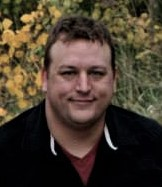
\includegraphics[width=0.3\textwidth]{profile2.jpg}
\caption{\label{fig:Me}This is a picture of me.}
\end{figure}

\section{Git repository location and learning this week}

\subsection{GitHub repository location with source code}

The GitHub repository that I have used is the one that I have created under the boultclass group. I plan to use 
this repo for all the assignments for this course.

The repo for this assignment may be found at:
\href{https://github.com/BoultClasses/dstout}{https://github.com/BoultClasses/dstout}

\subsection{What I have learned this week}

This week, I have been focusing on learning the necessary tools to do the homework for this class. I had very 
limited exposure to \LaTeX{} previously and have never used Overleaf before so I had to navigate the Overleaf 
interface and relearn a lot of the LaTex commands that I had previously used.I also had never heard of Zotero 
and had to learn how to use it to my benefit.

\subsubsection{Problems and struggles that were overcome}
The majority of problems that I had with this assignment came from my lack of knowledge with Zotero. In 
particular I found it difficult to create sufficient entries in the program itself. I overcame this problem by 
installing the chrome addon for Zotero that allowed entries to be made from a pdf with just the click of a 
button. The next big problem was figuring out how to create a .bib file from Zotero that could be used in the 
Overleaf project. After exporting the library, I was able to create the file in BibTex and watched a video on how to properly incorporate it.

Another issue that I had was pushing the Overleaf paper project directly to GitHub. I did not find a sufficient 
method to do so before the due date for this assignment and just did a work-around by downloading the project 
as a zipfile, which I could then manually push to my repo. I will continue my learning to be able to do this 
directly through Overleaf in the future.

\subsection{Papers - overview and formula}

\textbf{Are all code smells harmful? A study of God Classes and Brain Classes in the evolution of three open 
source systems.} 

\cite{olbrich_are_2010} The claim that classes that involved in certain code smells are liable to be changed 
frequently, having more defects than other classes is explored in this paper. They investigate the whether thi 
claim is true for God  and Brain Classes. The results show that God and Brain Classes were changed more 
frequently and contained more defects than other kinds of class, but when normalized for size the changes were 
less frequent.

The formula for detecting a God Class(GC) is as follows:
\[GC(C) = \begin{cases}
			1, & ((WMC(C) \geq 47) \wedge (TCC(C) < 0.\bar{3}) \wedge (ATFD(C) > 5)) \\
            0, & else
\end{cases}\]
Where: 
\begin{itemize}
\item C is the class being inspected.
\item Weighted Method Count (WMC(C)) is the sum of the cyclomatic complexity of all methods in C.
\item Tight Class Cohesion (TCC(C)) is the relative number of directly connected methods in C.
\item Access To Foreign Data (ATFD(C)) is the number of attributes of foreign classes accessed directly by class C or via accessor methods.
\end{itemize}

This formula was used by the authors in the detection strategy of God Classes for this paper. It established a base line by which a class could be considered a God Class and not a Brain class.


\textbf{Detecting and comparing brain activity in short program comprehension using EEG}

\cite{yeh_detecting_2017}The authors believe that programming comprehension comes at different stages of the SDLC. This is measured using EEG analysis and then is plotted with ANOVA testing.

\textbf{Java quality assurance by detecting code smells}

\cite{emden_java_2002}
The authors explore how the quality of code can be assessed automatically by checking for the presence of code smells. The feasibility of the approach is used in the design of a prototype tool that is applied to their case study successfully.

\textbf{Prevalence of confusing code in software projects: atoms of confusion in the wild}

\cite{gopstein_prevalence_2018}
The authors build on their previous atoms of confusion work to identify how these confusing micro patterns affect project level code and the rate of removal of these patterns in bug-repair commits. 

\textbf{Understanding misunderstandings in source code}

\cite{gopstein_understanding_2017}
The authors set out to identify inherently confusing micro patterns in code that can lead to runtime errors. The patterns are generally used in 
software projects and style guides, but they tend to confuse programmers. Using the authors identified confusing code, they show that in experiment they can lead to a significant increased rate of misunderstanding versus an equivalent code without the pattern.

\bibliographystyle{IEEEtran}
\bibliography{Exported_Items}

\end{document}